\DiaryEntry{Integration - Symmetries}{2016-04-25}{Integrals}

We have a continuous function \(f\) which is even on the interval
\([-a, a]\) (\(a>0\)).

The integral

\[
I = \int_{-a}^a \frac{f(x)}{1 + e^x} dx
\]

can be simplified as follows. First, we can rewrite the integral as

\[
I = \int_{-a}^a \frac{f(x)}{1 + e^{-x}} dx
\]

by substituting \(x \rightarrow -x\) and using the fact that \(f(x)\) is
even (\(f(x) = f(-x)\) on the integration interval). Then we have

\[
2I = \int_{-a}^a \frac{f(x)}{1 + e^x} dx + \int_{-a}^a \frac{f(x)}{1 + e^{-x}} dx = \int_{-a}^a f(x) \left( \frac{1}{1 + e^x} + \frac{1}{1 + e^{-x}} \right) dx
\]

which simplifies to

\[
2I =  \int_{-a}^a f(x) dx = 2 \int_{0}^a f(x) dx
\]

again using the evenness of \(f(x)\). This means that we have

\[
\int_{-a}^a \frac{f(x)}{1 + e^x} dx = \int_{0}^a f(x) dx
\]

\subsubsection{Example}

Consider the following integral

\[
I = \int_{-\pi/2}^{\pi/2} \frac{\cos x}{1+e^{x}} dx
\]

The function \(\cos x\) is even, therefore we can use the trick
mentioned above. Therefore, we have

\[
I = \int_0^{\pi/2} \cos x dx = \sin x \Big|_0^{\pi/2} = 1
\]

The Figure below shows the plot of the two integrands: red = original
expression, blue = simplified expression. Note that the integration
interval of the simplified expression is half the interval of the
complicated expression.

It is interesting to note that such a complicated expression and plot
can be simplified to such a great extent. On the other hand, it is
\textbf{just} the value of the integral which stays constant - it is
less surprising that two functions which look differently yield the same
integral value.

\begin{figure}
\centering
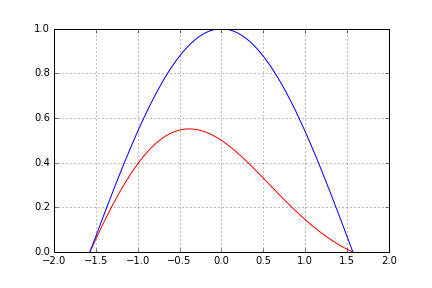
\includegraphics{images/integration-symmetries.png}
\end{figure}
